\documentclass[tikz,dvipdfmx]{standalone}

\usepackage{amsmath, amssymb, amsthm, mathrsfs, amsfonts, dsfont}
\usepackage{mathtools}
\usepackage{ifthen}

\usetikzlibrary{3d,arrows.meta,calc}

\definecolor{cA}{HTML}{0072BD}
\definecolor{cB}{HTML}{EDB120}
\definecolor{cC}{HTML}{77AC30}
\definecolor{cD}{HTML}{D95319}

\begin{document}
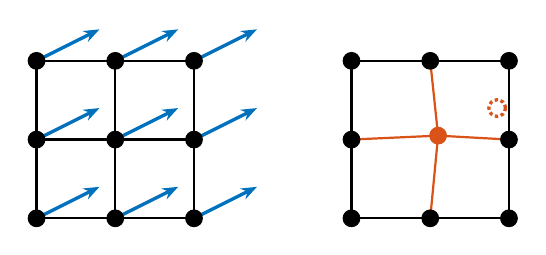
\begin{tikzpicture}
  \foreach \kind/\xS in {
      0/0,
      1/4
    }{
      \begin{scope}[xshift=\xS cm]
        \coordinate (a00) at (-1, 1);
        \coordinate (a01) at (-1, 0);
        \coordinate (a02) at (-1,-1);
        \coordinate (a10) at ( 0, 1);
        \coordinate (a12) at ( 0,-1);
        \coordinate (a20) at ( 1, 1);
        \coordinate (a21) at ( 1, 0);
        \coordinate (a22) at ( 1,-1);


        \ifthenelse{\equal{\kind}{0}}{
        \coordinate (a11) at ( 0, 0);
        \draw[-{Stealth[length=2mm]},very thick,cA] (a00) -- ($(a00)+(0.8,0.4)$);
        \draw[-{Stealth[length=2mm]},very thick,cA] (a01) -- ($(a01)+(0.8,0.4)$);
        \draw[-{Stealth[length=2mm]},very thick,cA] (a02) -- ($(a02)+(0.8,0.4)$);
        \draw[-{Stealth[length=2mm]},very thick,cA] (a10) -- ($(a10)+(0.8,0.4)$);
        \draw[-{Stealth[length=2mm]},very thick,cA] (a11) -- ($(a11)+(0.8,0.4)$);
        \draw[-{Stealth[length=2mm]},very thick,cA] (a12) -- ($(a12)+(0.8,0.4)$);
        \draw[-{Stealth[length=2mm]},very thick,cA] (a20) -- ($(a20)+(0.8,0.4)$);
        \draw[-{Stealth[length=2mm]},very thick,cA] (a21) -- ($(a21)+(0.8,0.4)$);
        \draw[-{Stealth[length=2mm]},very thick,cA] (a22) -- ($(a22)+(0.8,0.4)$);
        }{
        \coordinate (a11) at ( 0.1, 0.05);
        }

        \draw[thick] (a00) -- (a01);
        \draw[thick] (a01) -- (a02);
        \draw[thick] (a20) -- (a21);
        \draw[thick] (a21) -- (a22);
        \draw[thick] (a00) -- (a10);
        \draw[thick] (a10) -- (a20);
        \draw[thick] (a02) -- (a12);
        \draw[thick] (a12) -- (a22);

        \ifthenelse{\equal{\kind}{0}}{
          \draw[thick] (a10) -- (a11);
          \draw[thick] (a11) -- (a12);
          \draw[thick] (a01) -- (a11);
          \draw[thick] (a11) -- (a21);
        }{
          \draw[thick,cD] (a10) -- (a11);
          \draw[thick,cD] (a11) -- (a12);
          \draw[thick,cD] (a01) -- (a11);
          \draw[thick,cD] (a11) -- (a21);
        }

        \filldraw[draw=black,fill=black] (a00) circle (3pt);
        \filldraw[draw=black,fill=black] (a01) circle (3pt);
        \filldraw[draw=black,fill=black] (a02) circle (3pt);
        \filldraw[draw=black,fill=black] (a10) circle (3pt);
        \filldraw[draw=black,fill=black] (a12) circle (3pt);
        \filldraw[draw=black,fill=black] (a20) circle (3pt);
        \filldraw[draw=black,fill=black] (a21) circle (3pt);
        \filldraw[draw=black,fill=black] (a22) circle (3pt);

        \ifthenelse{\equal{\kind}{0}}{
          \filldraw[draw=black,fill=black] (a11) circle (3pt);
        }{
          \filldraw[draw=cD,fill=cD] (a11) circle (3pt);
          \draw[very thick,cD,densely dotted] ($(a11)+(0.75,0.35)$) circle (3pt);
        }
      \end{scope}
    }
\end{tikzpicture}
\end{document}